\begin{center}
  \Large
  \textbf{BIOGRAFI PENULIS}
\end{center}

\addcontentsline{toc}{chapter}{BIOGRAFI PENULIS}

\vspace{2ex}

\begin{wrapfigure}{L}{0.3\textwidth}
  \centering
  \vspace{-3ex}
  % Ubah file gambar berikut dengan file foto dari mahasiswa
  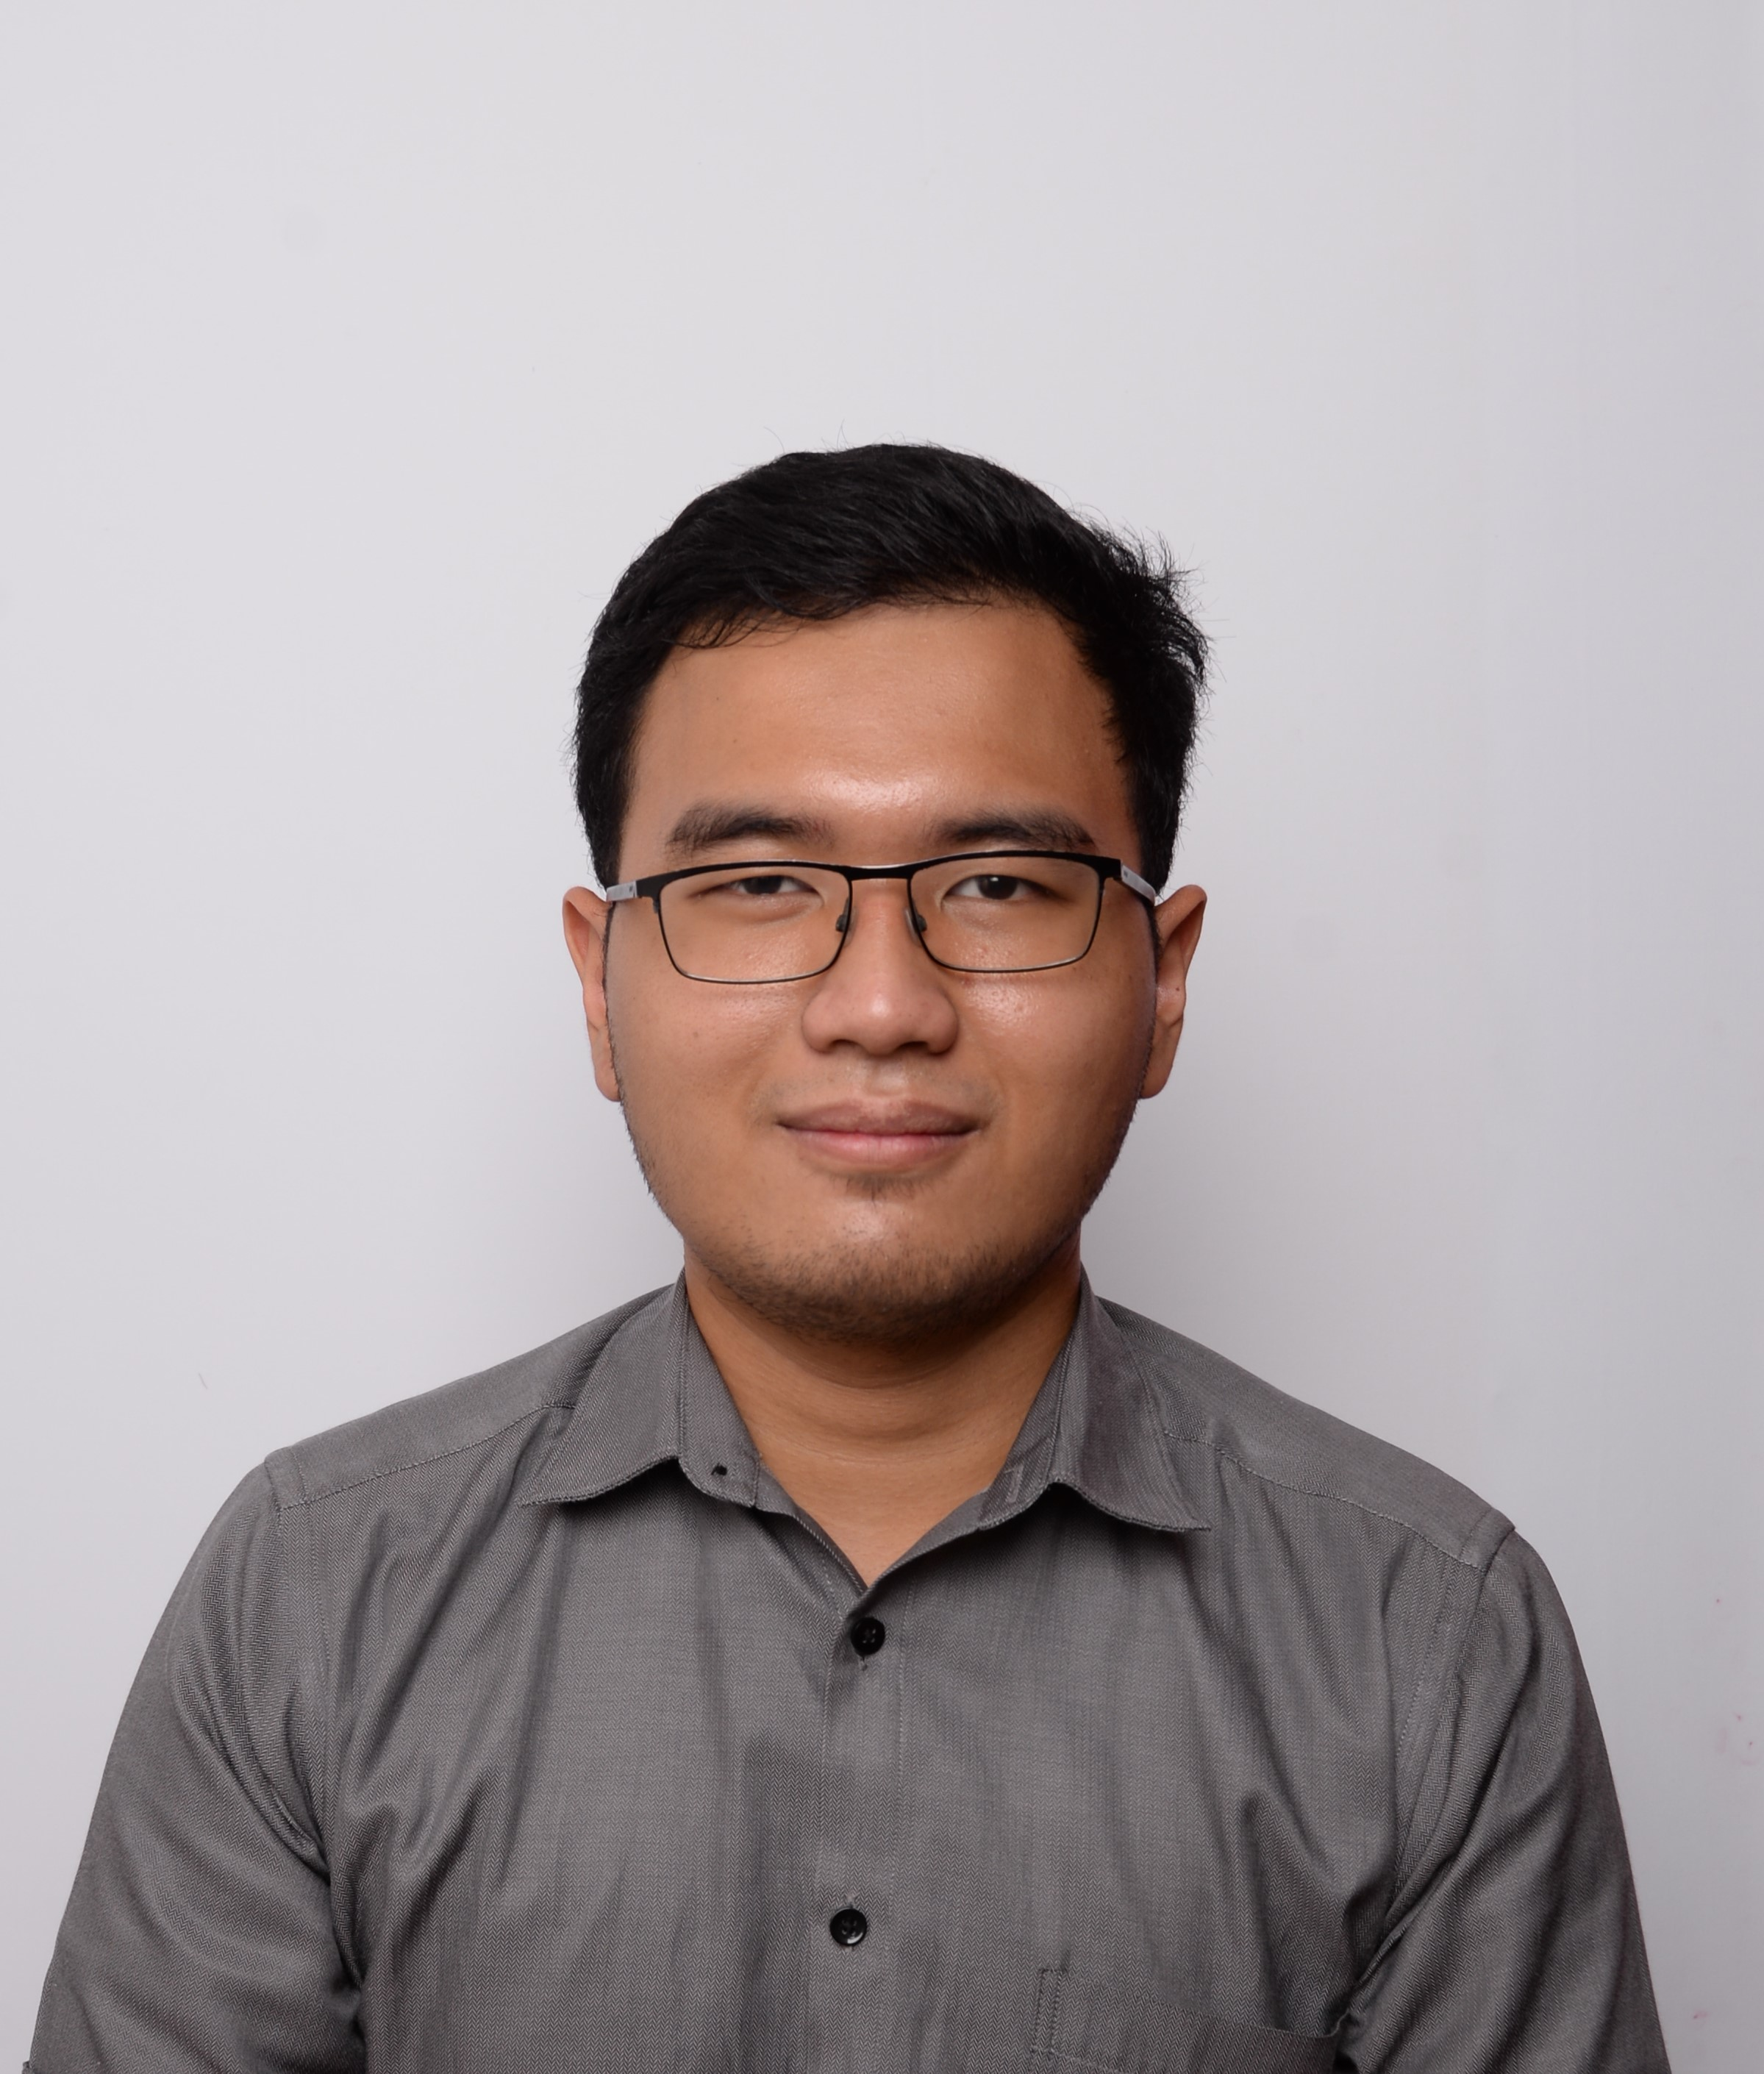
\includegraphics[width=0.3\textwidth]{gambar/bener/Foto Muhammad Daffa Z3.JPG}
  \vspace{-4ex}
\end{wrapfigure}

% Ubah kalimat berikut dengan biografi dari mahasiswa
Muhammad Daffa ZW, lahir di Jakarta pada 17 April 2001 , Merupakan seorang alumni dari Departemen Teknik Komputer Institut Teknologi Sepuluh Nopember (ITS) Surabaya . Menempuh Pendidikan Dasar di SDIT Ar Ridho , Pondok Kelapa , Jakarta Timur lalu melanjutkan pendidikan menengah pertama di SMPIT Ar Rudho , Pondok Kelapa , Jakarta timur lalu mengambil pendidikan menengah atas yaitu Madrasah Aliyah Negeri (MAN) 9 Jakarta dengan jurusan IPA yang berlokasi di Pondok Bambu , Jakarta Timur . Penulis memiliki minat dan hobi yang tinggi terhadap dunia Teknologi baik itu Perkembangan Teknologi Informasi seperti perkembangan teknologi software yang lagi terkenal saat ini baik itu di bidang Software Engineering , Artificial Intelligence , dll sebagainya , Selain itu penulis juga memiliki minat yang tinggi terhadap bidang Sejarah , Militer dan Geopolitik , Karena penulis sangat menyukai permainan video yang berbau peperangan seperti Call Of Duty , Insurgency , Battlefield dll sehingga penulis sangat memiliki minat yang tinggi terhadap dunia militer dan juga hal hal yang terkait dengan hal itu seperti Sejarah karena dengan hal ini kita bisa memahami dan mengerti lebih lagi terkait kenapa hal ini terjadi , kenapa hal ini begitu dan lain sebagai nya . Minat dan Hobi ini yang sering dituangkan dalam bentuk tulisan-tulisan pikiran yang biasa tulis di jejaring sosial seperti Facebook , Instagram dll sebagainya 

